\documentclass[dvipdfmx]{standalone}
\usepackage{tikz}

\begin{document}
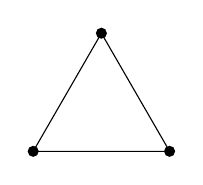
\begin{tikzpicture}
    % 頂点を定義 (座標は極座標: 角度:距離 で指定すると正三角形が作りやすい)
    % 90度、210度(90+120)、330度(210+120) の位置に配置
    \coordinate (A) at (90:1);
    \coordinate (B) at (210:1);
    \coordinate (C) at (330:1);

    % 頂点を黒丸で描画
    \fill (A) circle (2pt);
    \fill (B) circle (2pt);
    \fill (C) circle (2pt);

    % 辺を描画 (cycle で始点に戻って閉じる)
    \draw (A) -- (B) -- (C) -- cycle;
\end{tikzpicture}
\end{document}